\documentclass[xcolor=table, 10pt, aspectratio=169]{beamer}

%\usepackage{arev}
\usepackage{amsmath,amssymb,amscd}
\usepackage{dsfont}
\usepackage{mathrsfs}
\usepackage{yfonts}
\usepackage{bm}
\usepackage{graphicx}
\usepackage{tabularx}
\usepackage{animate}
%\usepackage{mathtools}
%\usepackage{ifthen}

%\usepackage{xeCJK}
%\usepackage{fontspec}
%\newfontfamily\cjkfont{PingFang SC}
%\setCJKmainfont{PingFang SC}
\newcolumntype{x}{>{\centering\arraybackslash}X}
\renewcommand{\arraystretch}{1.5}

\usepackage{tikz}
	\usetikzlibrary{calc}
	\usetikzlibrary{arrows,shapes, positioning, matrix}
	\usetikzlibrary{decorations.markings}
	\tikzset{>=stealth}
	\tikzstyle arrowstyle=[scale=1]
	\tikzstyle directed=[postaction={decorate,decoration={markings,
 	   mark=at position .15 with {\arrow[arrowstyle]{stealth}}}}]
\tikzstyle string=[thick,postaction={decorate,decoration={markings,
    mark=at position .55 with {\arrow[arrowstyle]{stealth}}}}]
\tikzstyle dual_string=[dashed,postaction={decorate,decoration={markings,
    mark=at position .55 with {\arrow[arrowstyle]{stealth}}}}]

\tikzstyle dw=[thick,postaction={decorate,decoration={markings,
    mark=at position 1 with {\arrow[arrowstyle]{stealth}}}}]
\tikzstyle group=[mbg]
\newcommand*{\halfway}{0.5*\pgfdecoratedpathlength+.5*8pt}\tikzstyle arrowstyle=[scale=1]
\newcommand*{\halfwayb}{0.5*\pgfdecoratedpathlength}
\tikzstyle arrowstyle=[scale=1]
\tikzstyle fermion=[thick,postaction={decorate},decoration={markings,
    mark=at position \halfway with {\arrow[arrowstyle]{latex}}}]
\tikzstyle fermion2=[thick,postaction={decorate},decoration={markings,
        mark=at position \halfwayb with {\arrow[arrowstyle]{latex}}}]

\usepackage{pgffor}
\newcommand{\mb}[1]{\mathbf{#1}}
\renewcommand{\cal}[1]{\mathcal{#1}}

\newcommand{\ag}[2]{#1_\mb{#2}}
\newcommand{\cohosub}[1]{\scalebox{0.72}{\textswab{#1}}}
\newcommand{\cohosubsub}[1]{\scalebox{0.6}{\textswab{#1}}}
\newcommand{\coho}[1]{\textswab{#1}}

\DeclareMathOperator{\tr}{Tr}
\DeclareMathOperator{\im}{Im}
\DeclareMathOperator{\re}{Re}

\mode<presentation>
{
  %\usetheme{Warsaw}
  % or ...
  %\useoutertheme{rectangle}
  \setbeamertemplate{frametitle}[default][center]
  \defbeamertemplate{itemize item}{flat}{\begin{pgfpicture}{-1ex}{0ex}{1ex}{2ex}
      \pgfpathcircle{\pgfpoint{0pt}{.6ex}}{0.6ex}
      \pgfusepath{fill}
    \end{pgfpicture}%
  }
  \defbeamertemplate{itemize subitem}{flat}{\footnotesize\raise0.5pt\hbox{\textbullet}}
  \defbeamertemplate{itemize subsubitem}{flat}{\footnotesize\raise0.5pt\hbox{\textbullet}}

  %\useinnertheme{circles}
  \setbeamertemplate{items}[flat]
  \setbeamertemplate{sections/subsections in toc}[circle]
  \setbeamertemplate{blocks}[rounded]
  \setbeamertemplate{title page}[default][colsep=-4bp,rounded=true]
  \setbeamertemplate{part page}[default][colsep=-4bp,rounded=true]
  \setbeamercovered{transparent}
  %\usecolortheme{spruce}
  %\definecolor{THU}{RGB}{116,61,130}
  \definecolor{mbg}{RGB}{0,0,160}
  \setbeamercolor*{palette primary}{fg=white,bg=mbg}
  \setbeamercolor*{titlelike}{parent=palette primary}
  \setbeamercolor*{structure}{fg=mbg}
  \setbeamercolor{frametitle}{fg=white,bg=mbg}
  % or whatever (possibly just delete it)
  \setbeamercolor{block title}{bg=mbg,fg=white}
  \setbeamercolor{block body}{bg=mbg!15}


  \addtobeamertemplate{navigation symbols}{}{ \hspace{1em}%
    \usebeamerfont{footline}%
    \insertframenumber / \inserttotalframenumber }
}


%\usepackage[english]{babel}
% or whatever

%\usepackage[latin1]{inputenc}
% or whatever

%\usepackage{times}
%\usepackage[T1]{fontenc}
% Or whatever. Note that the encoding and the font should match. If T1
% does not look nice, try deleting the line with the fontenc.

\title[Fermi Arcs] % (optional, use only with long paper titles)
{Fermi Arcs in Anderson Lattice Models w/ d-wave Hybridization}

\author[Y Qi] % (optional, use only with lots of authors)
{Yang~Qi}
% - Give the names in the same order as the appear in the paper.
% - Use the \inst{?} command only if the authors have different
%   affiliation.

\institute[Fudan] % (optional, but mostly needed)
{Department of Physics, Fudan University}
% - Use the \inst command only if there are several affiliations.
% - Keep it simple, no one is interested in your street address.

%\date{2016 Annual Meeting of Fudan CFTPP} % (optional, should be abbreviation of conference name)
%{Fudan University, Oct 13 2015}
\date{16th BFHTS, 2018.}
% - Either use conference name or its abbreviation.
% - Not really informative to the audience, more for people (including
%   yourself) who are reading the slides online

\subject{Theoretical Physics}
% This is only inserted into the PDF information catalog. Can be left
% out.



% If you have a file called "university-logo-filename.xxx", where xxx
% is a graphic format that can be processed by latex or pdflatex,
% resp., then you can add a logo as follows:

%\pgfdeclareimage[height=1cm]{university-logo}{fudan}
%\logo{\pgfuseimage{university-logo}}



% Delete this, if you do not want the table of contents to pop up at
% the beginning of each subsection:

\begin{document}

\begin{frame}
  \titlepage
\end{frame}

\begin{frame}{References}
\begin{itemize}
%\item Works led by Liang Fu, Zi-Yang Meng, and Lei Wang.
\item MIT: Vladyslav Kozii, Hiroki Isobe, Liang Fu.
\item CCSE, Japan Atomic Energy Agency: Yuki Nagai.
\begin{center}
	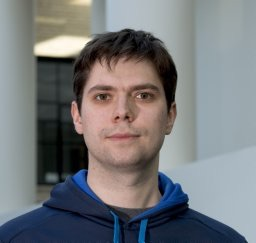
\includegraphics[height=3cm]{../people/vlad}
	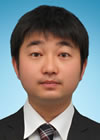
\includegraphics[height=3cm]{../people/yuki}
	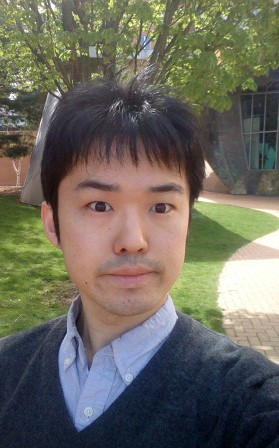
\includegraphics[height=3cm]{../people/hiroki}
	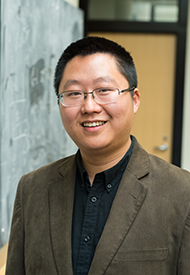
\includegraphics[height=3cm]{../people/liangfu}
\end{center}
\item Working in progress.
\end{itemize}
\end{frame}

%\begin{frame}
%\frametitle{Kondo physics from non-Hermitian Hamiltonian}
%\begin{itemize}
%\item Consider a two-band model,
%\[H_0=\sum_k\begin{pmatrix}f_{k\alpha}^\dagger&c_{k\alpha}^\dagger\end{pmatrix}
%\begin{pmatrix}\epsilon_{fk} & V_k\\ V_k & \epsilon_{ck}\end{pmatrix}
%\begin{pmatrix}f_{k\alpha}\\c_{k\alpha}\end{pmatrix}.\]
%\item With two lifetimes,
%\[G^{-1}(k,\omega)=\omega-H_0(k)-\Sigma_k,\quad
%\Sigma_k=-i\begin{pmatrix}\Gamma_f & 0\\0 & \Gamma_c\end{pmatrix}.\]
%\item Non-Hermition effective Hamiltonian,
%\[H = H_0+\Sigma = \begin{pmatrix}
%\epsilon_{fk} - i\Gamma_f & V_k\\ V_k & \epsilon_{ck} - i\Gamma_c
%\end{pmatrix}, \quad G=(\omega-H)^{-1}.\]
%\end{itemize}
%Vlad Kozii and Liang Fu, arXiv:1708.05841.
%\end{frame}

\begin{frame}
\frametitle{Kondo physics from non-Hermitian Hamiltonian}
\begin{itemize}
\item The non-Hermitian quasiparticle Hamiltonian $H = H_0+\Sigma = \begin{pmatrix}
\epsilon_{fk} - i\Gamma_f & V_k\\ V_k & \epsilon_{ck}
\end{pmatrix}$.
\item Electron spectrum density
\[A(k, \omega)=-\frac1\pi\tr\im (\omega - H)^{-1}
=-\frac2\pi\im\left(
\frac1{\omega-E_1}+\frac1{\omega-E_2}\right)
=\frac2\pi\sum_{a=1,2}\frac{\im E_a}{(\omega-\re E_a)^2+\im E_a^2}.\]
\item Exceptional point: $|V_k|=\Gamma_f$, where $E_1=E_2$.
\end{itemize}

\begin{columns}
\column{.65\textwidth}
\begin{itemize}
\item Along $\epsilon_{ck}=\epsilon_{fk}=\mu$:
\item $|V_k|>\Gamma_f$: $\re E_1\neq\re E_2$, two peaks, gap open.\\
Low $T$: FS = $c+f$, Kondo insulator.
\item $|V_k|<\Gamma_f$: $\re E_1=\re E_2$, one peak, gap close.\\
High $T$: FS = $c$, Metal.
\end{itemize}
\column{.4\textwidth}
%\begin{center}
	%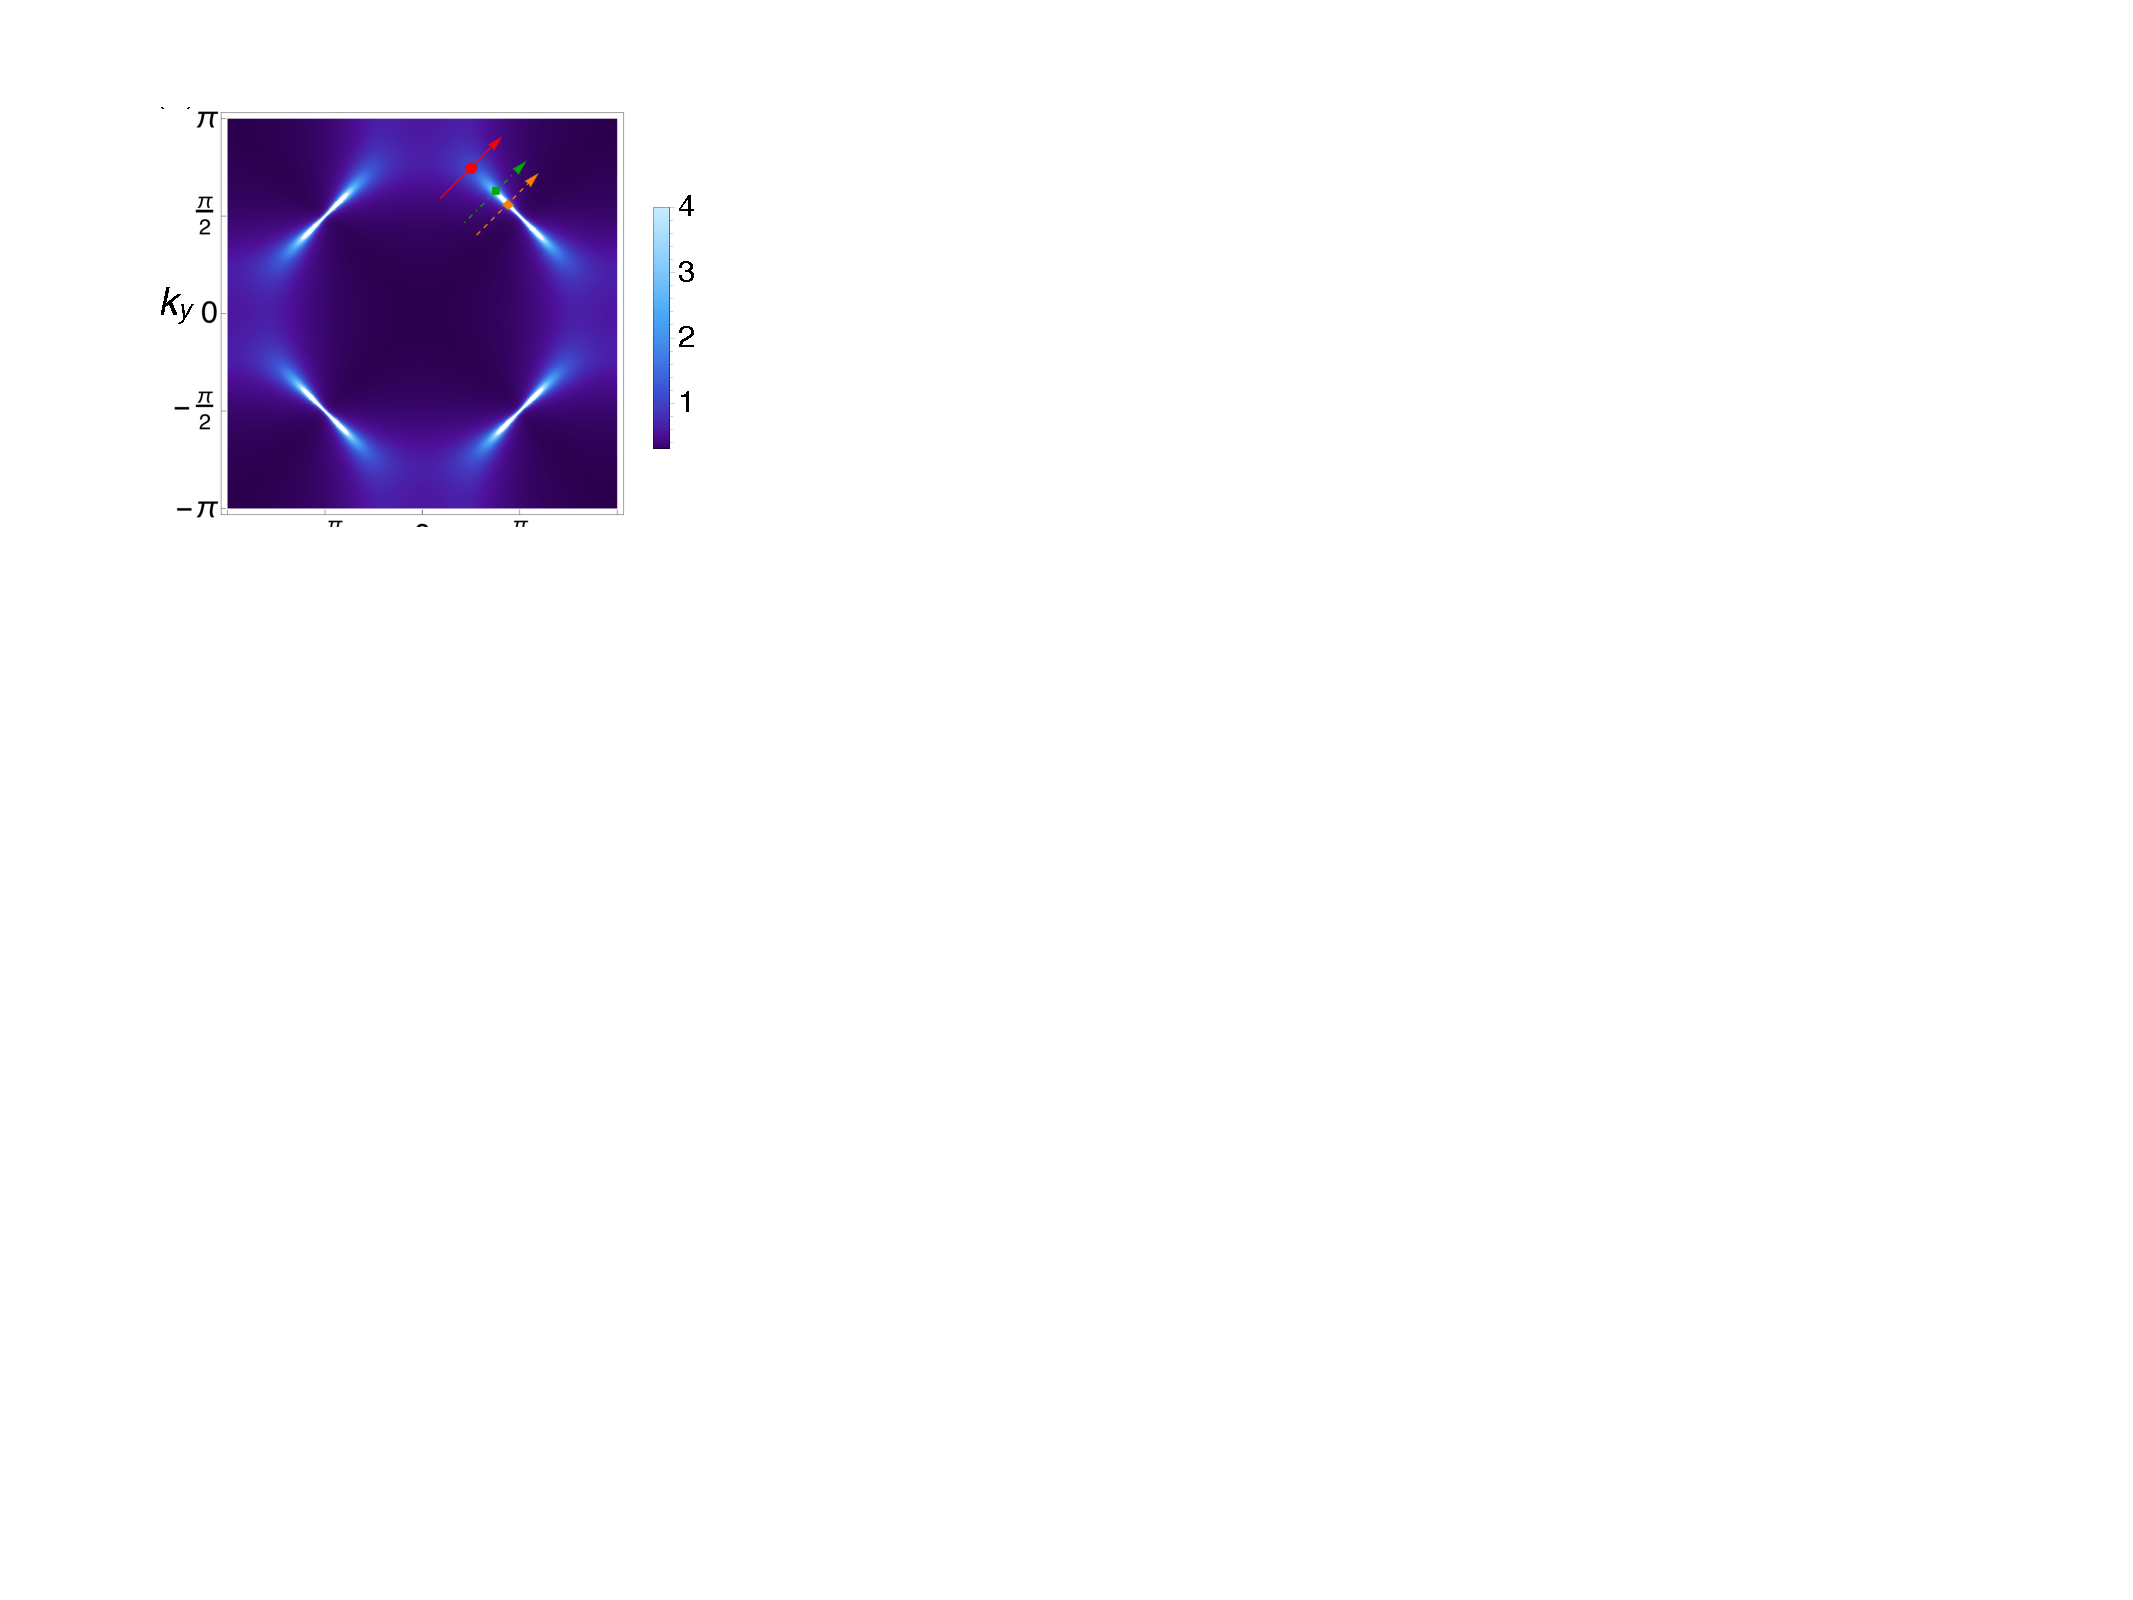
\includegraphics[height=2.5cm]{arc1}
	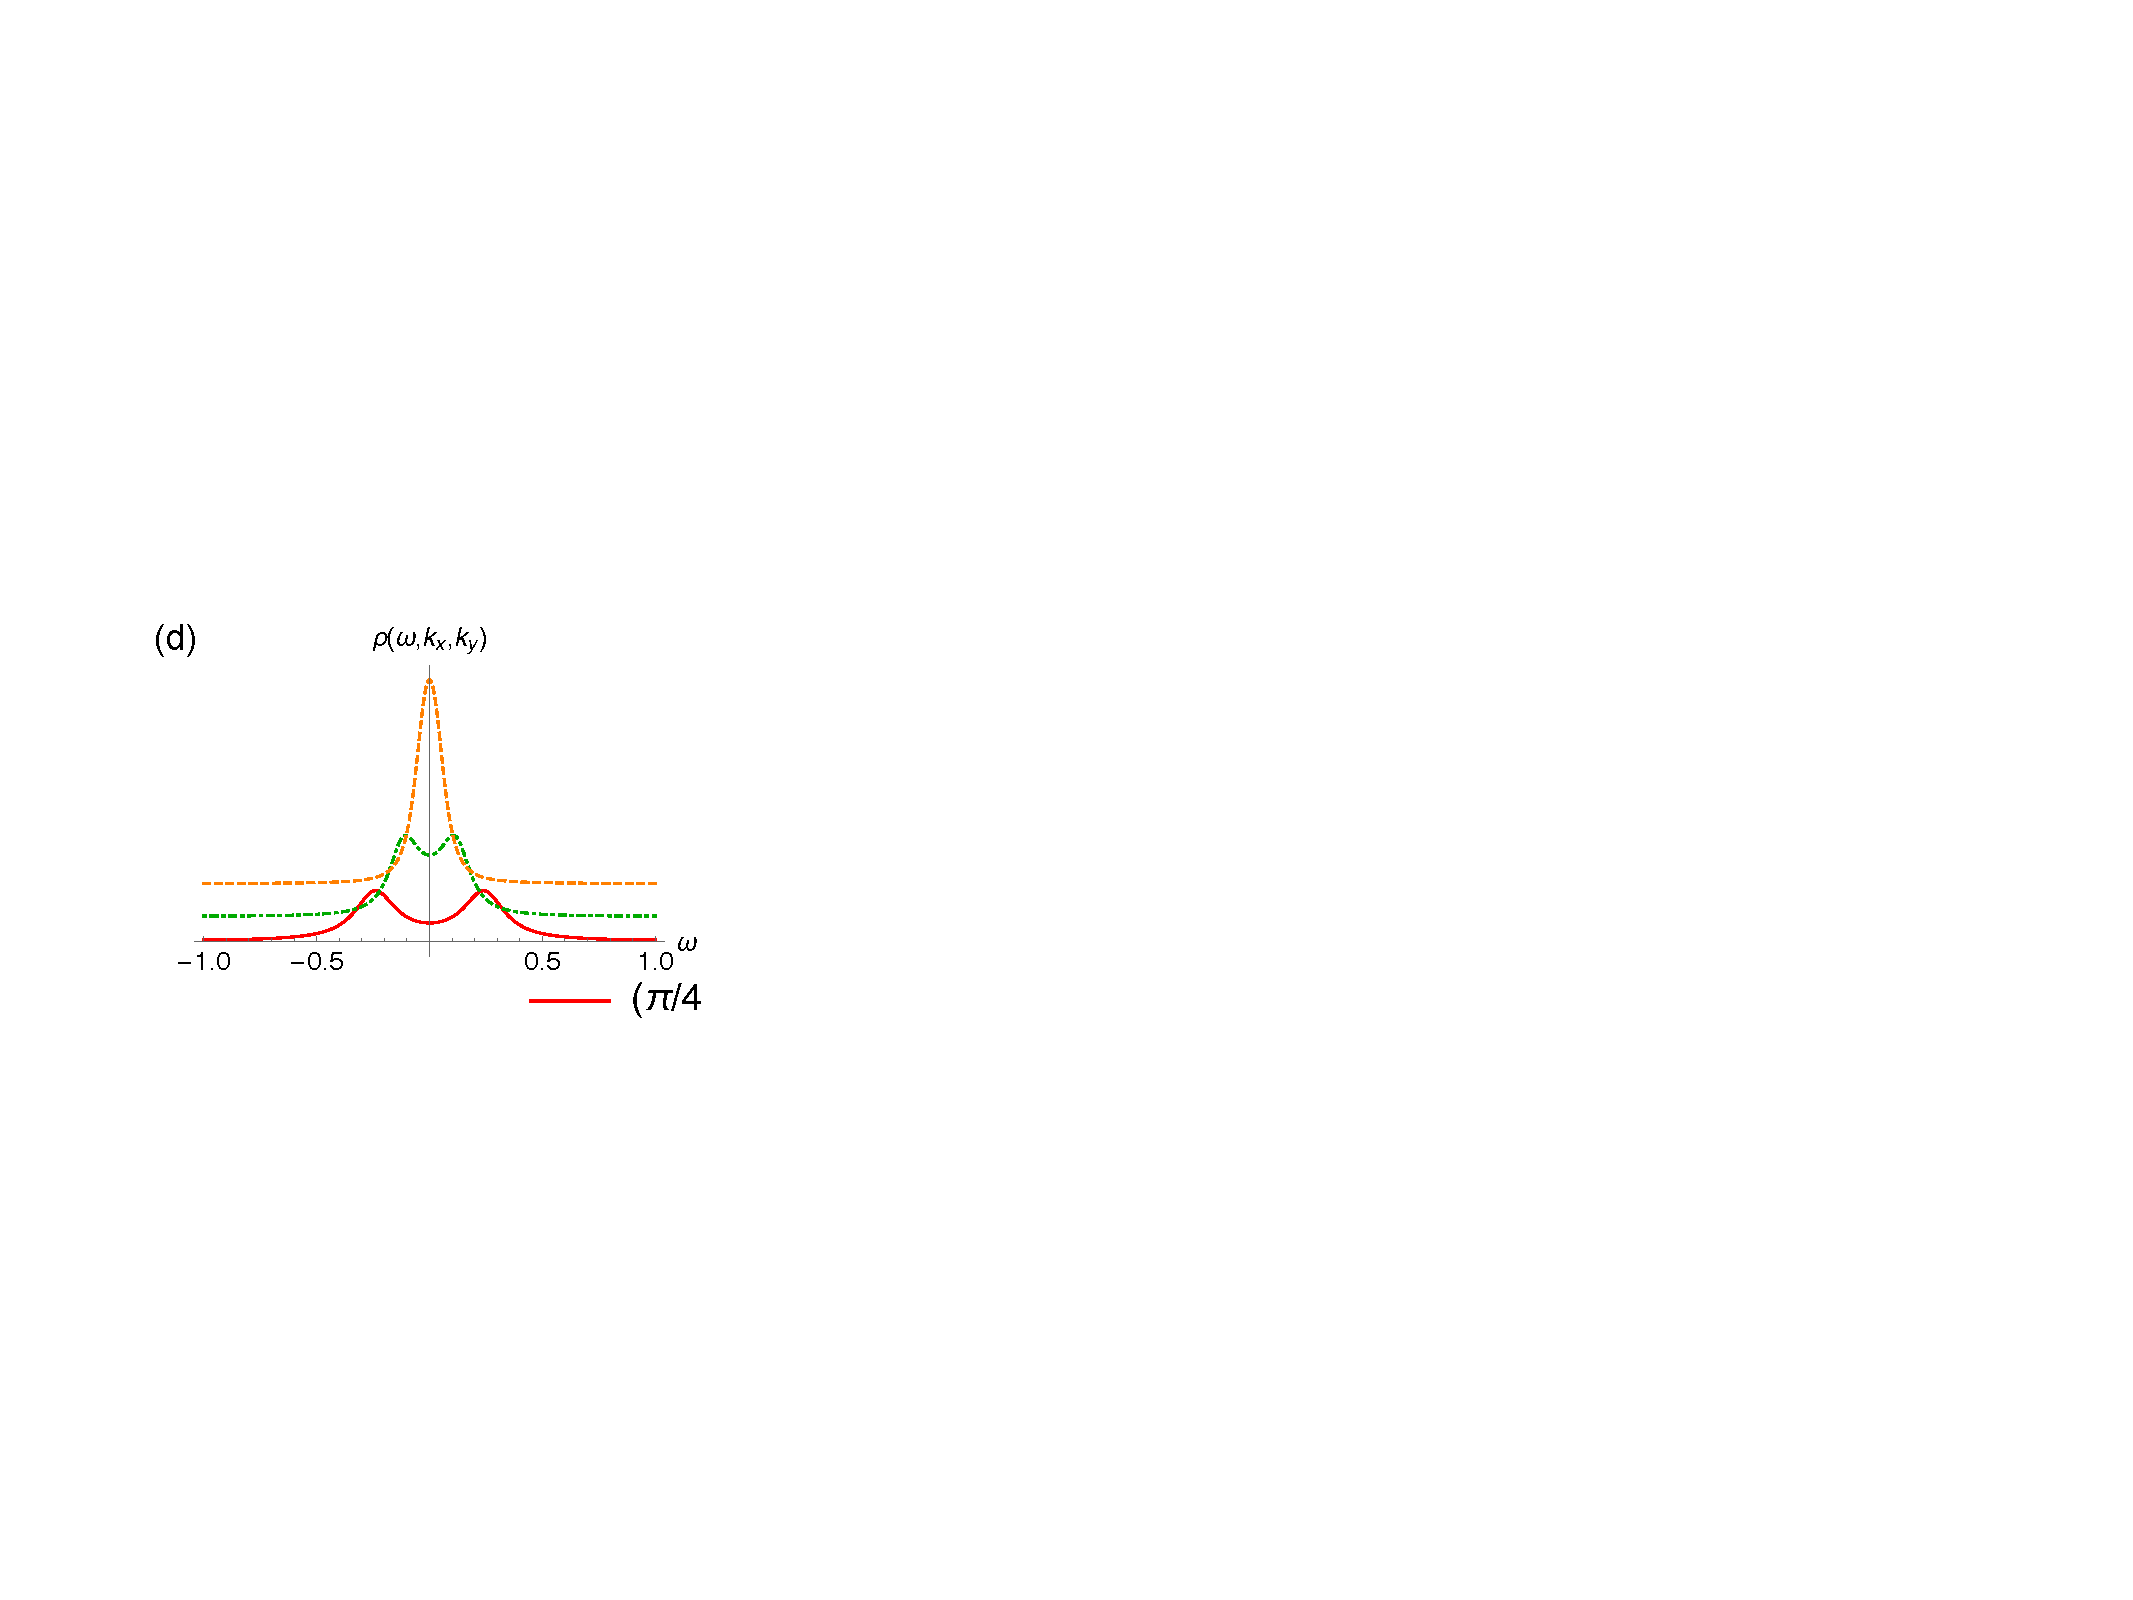
\includegraphics[height=4cm]{arc2}
%\end{center}
\end{columns}
\end{frame}

\begin{frame}
\frametitle{Fermi arcs as a result of d-wave hybridization}
\begin{itemize}
\item A $k$-dependent hybridization $V_k=V_0(\cos k_x+\cos k_y)$.
\item $\Gamma_f$ increases with temperature.
\item $|V_k|<\Gamma_f$: one peak = Fermi arc. Like a small Fermi surface.
\item $|V_k|>\Gamma_f$: two peaks = gapped. Like a Kondo insulator.
\item A dichotomy on the Fermi surface when $\Gamma_f<V_0$: separated by the exceptional points $|V_k|=\Gamma_f$.
\item Fermi arc grows with temperature.
\end{itemize}
\begin{center}
	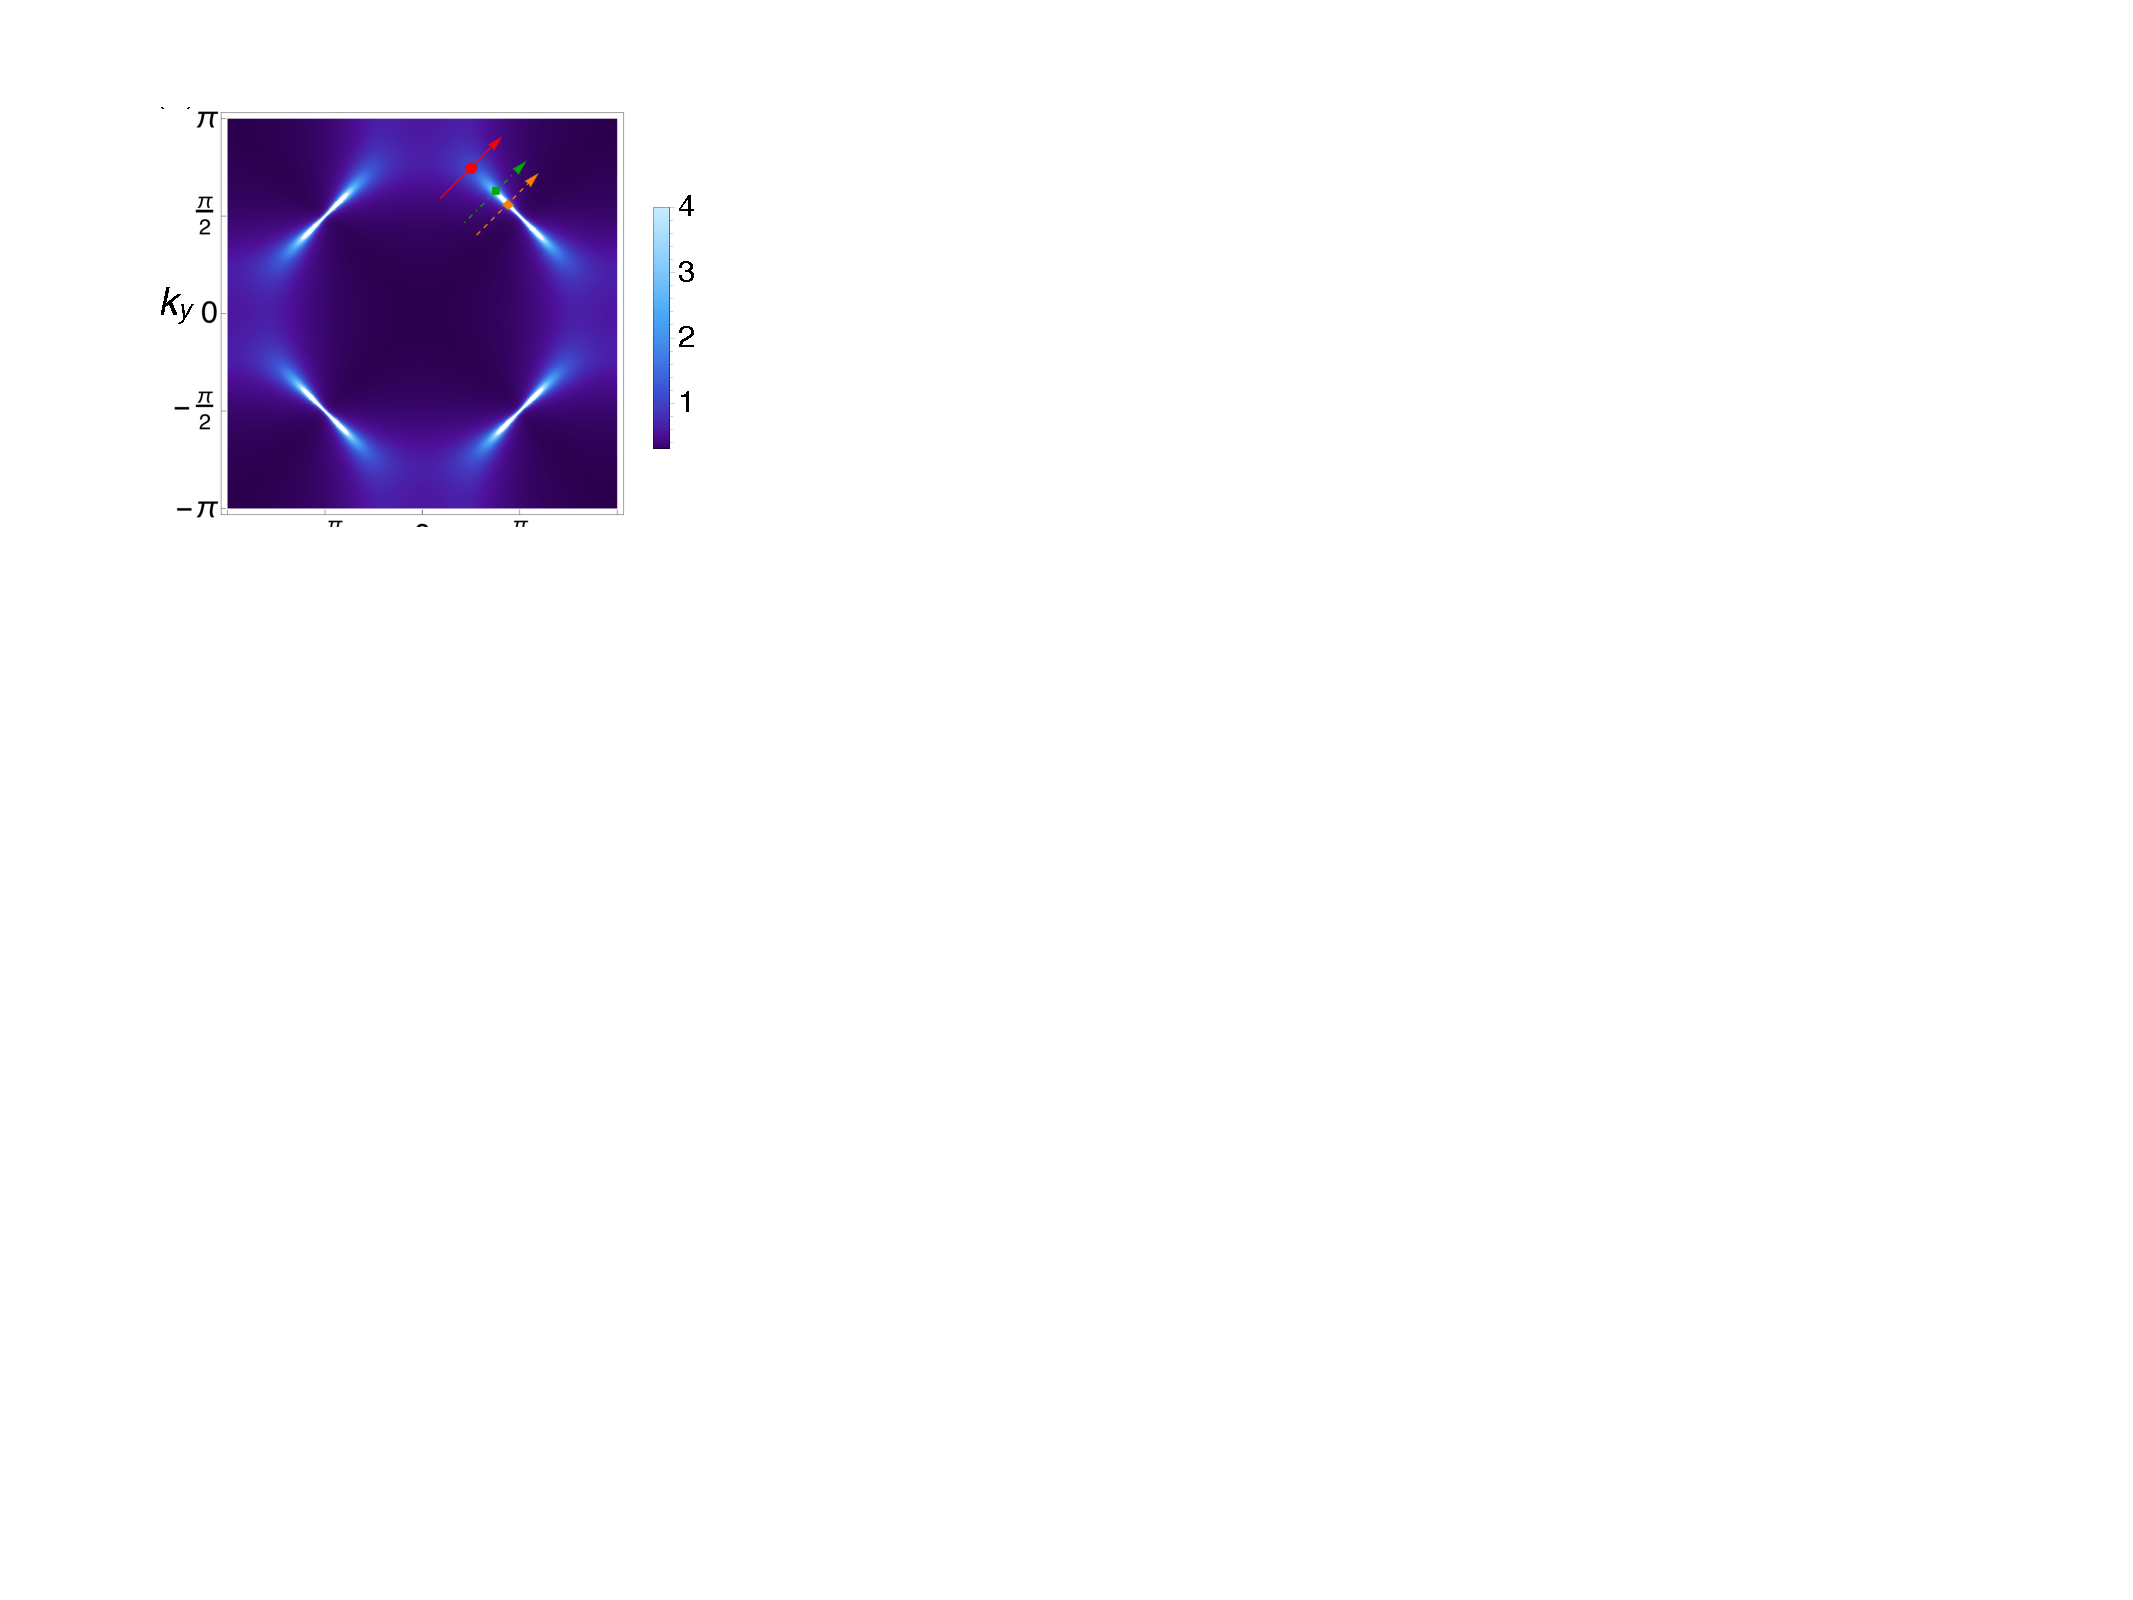
\includegraphics[height=3cm]{arc1}~~~~
	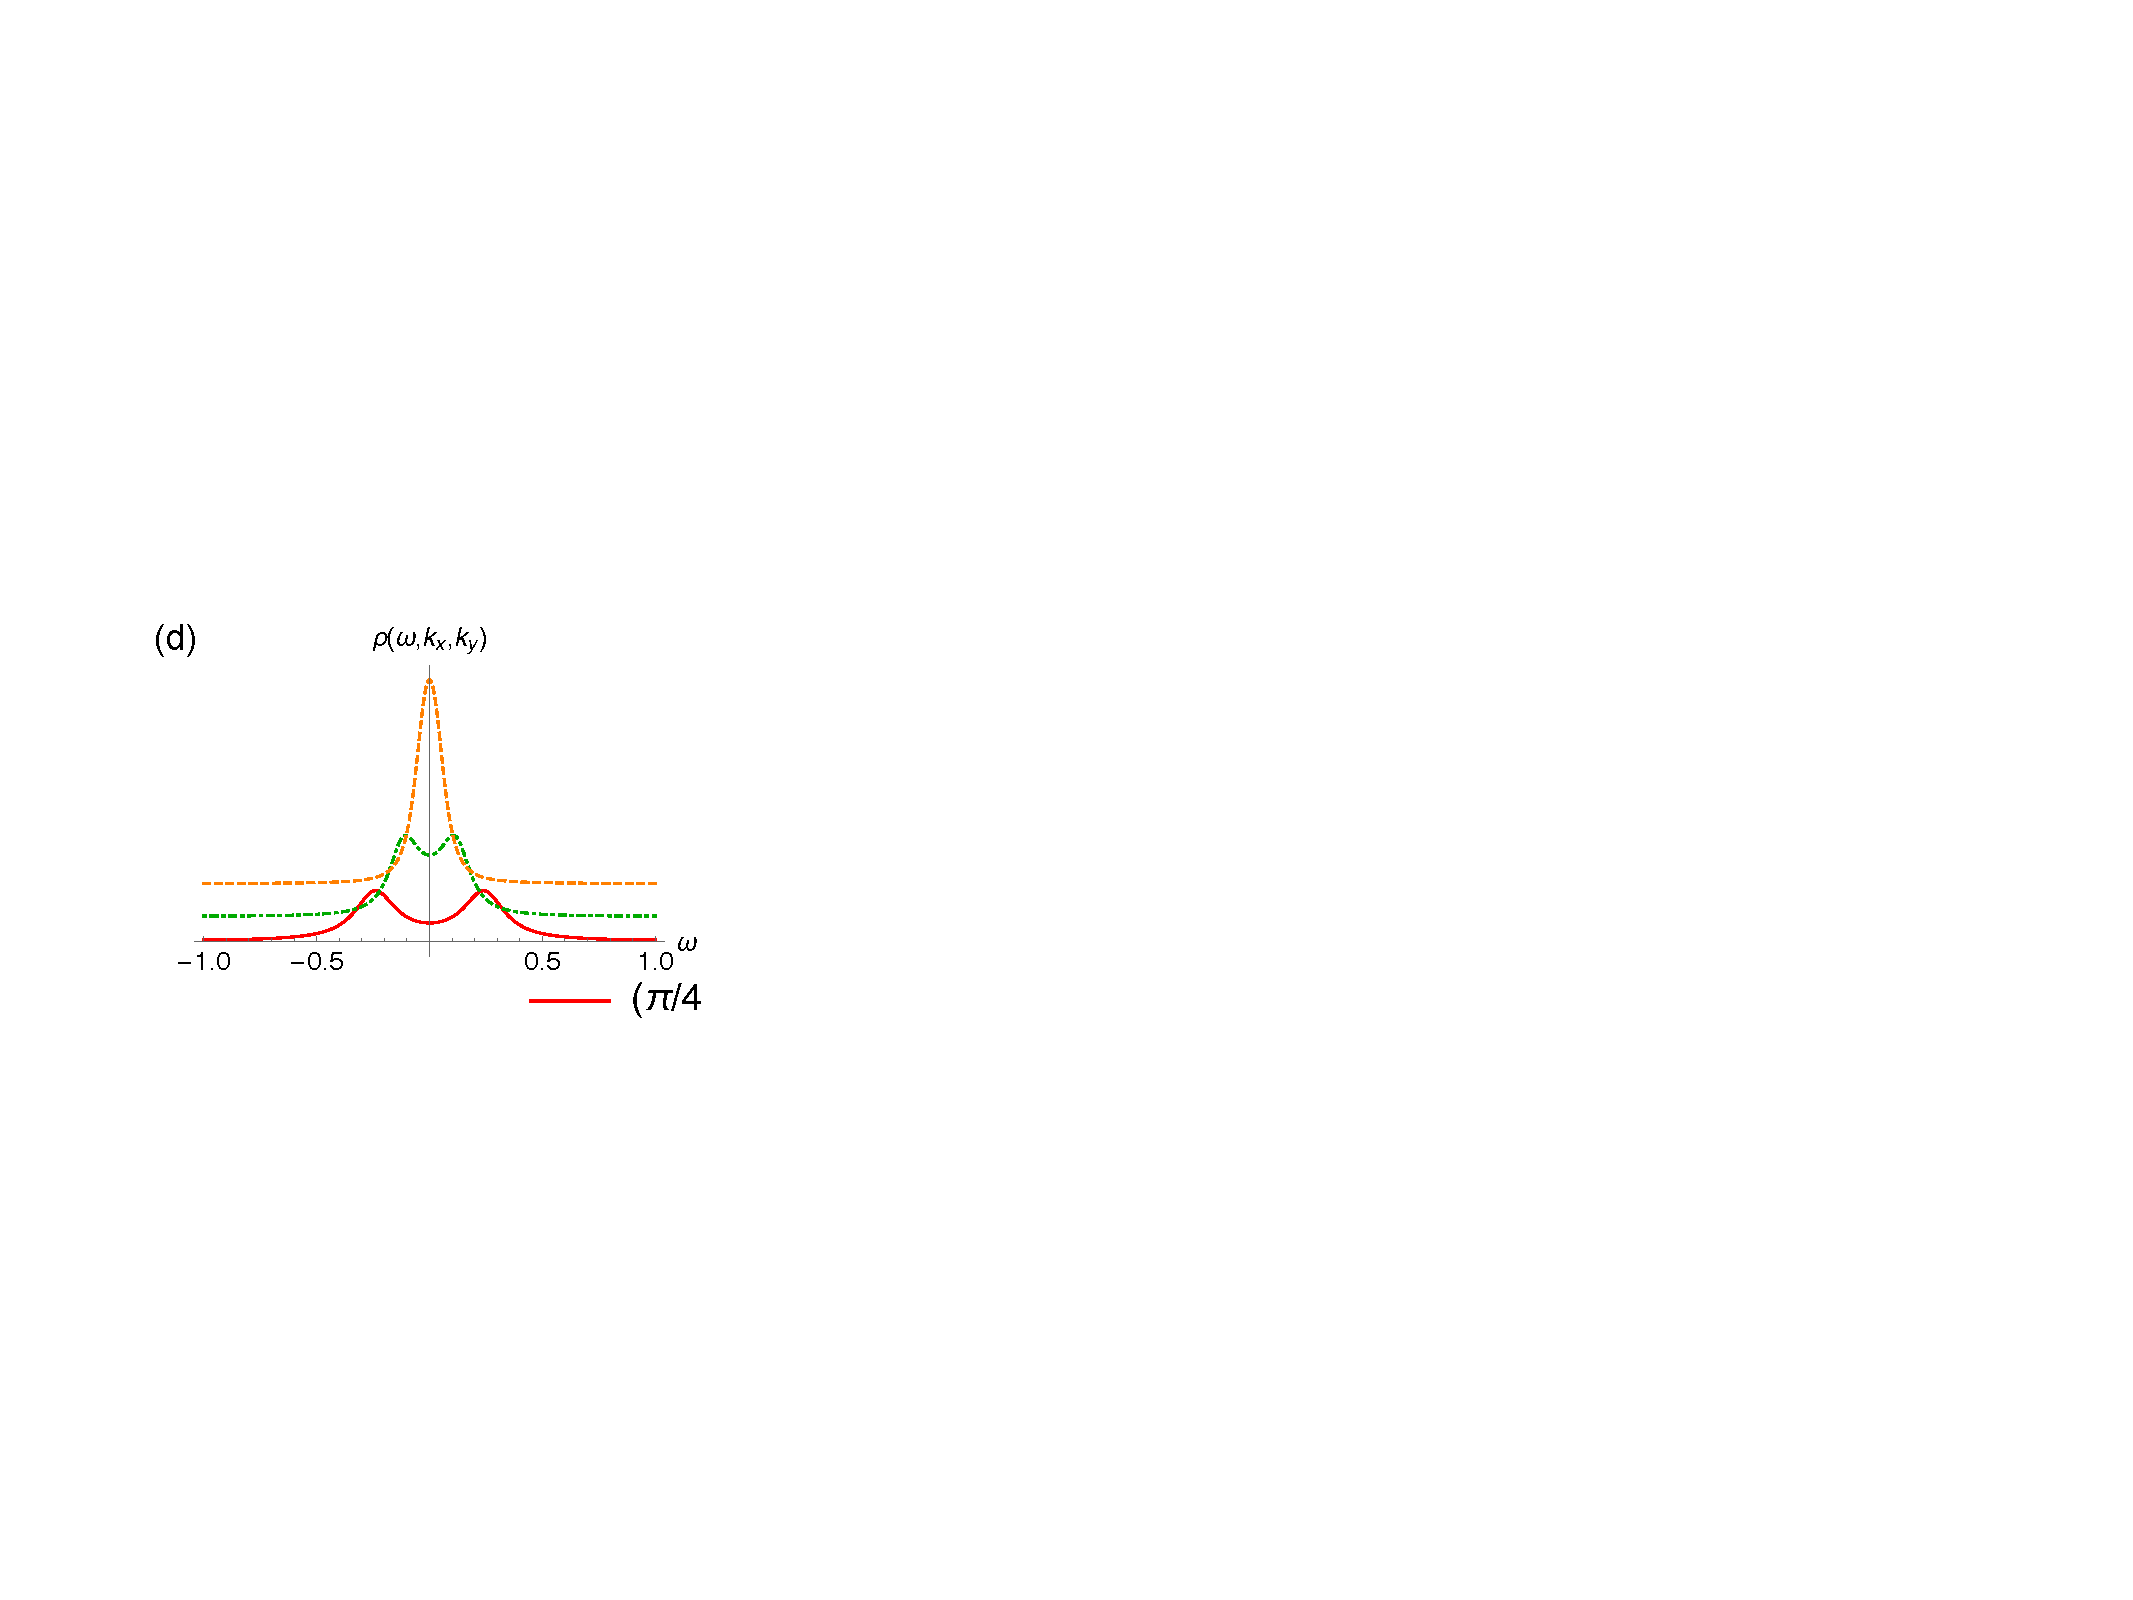
\includegraphics[height=3cm]{arc2}
\end{center}
\end{frame}


\begin{frame}
\frametitle{Summary of our work}
\begin{itemize}
\item<1-7> An Anderson-Lattice model w/ d-wave hybridization.
\item<2-5> We computed electron self energy using second-order perturbation theory and DMFT.
\item<3-8> $\Gamma_f\neq\Gamma_c=0$.
\item<4-6> At $T\geq v_0$, $\Sigma_f$ can be treated as a constant.
\item<5-9> $\Gamma_f\neq\Gamma_c$ and a $k$-dependent $V_k$ results in Fermi arcs:
\begin{enumerate}
\item $V_k<\Gamma_f$: one peak = Fermi arc. Like a small Fermi surface.
\item $V_k>\Gamma_f$: two peaks = gapped. Like a Kondo insulator.
\item A dichotomy on the Fermi surface.
\end{enumerate}
\end{itemize}
\begin{center}
	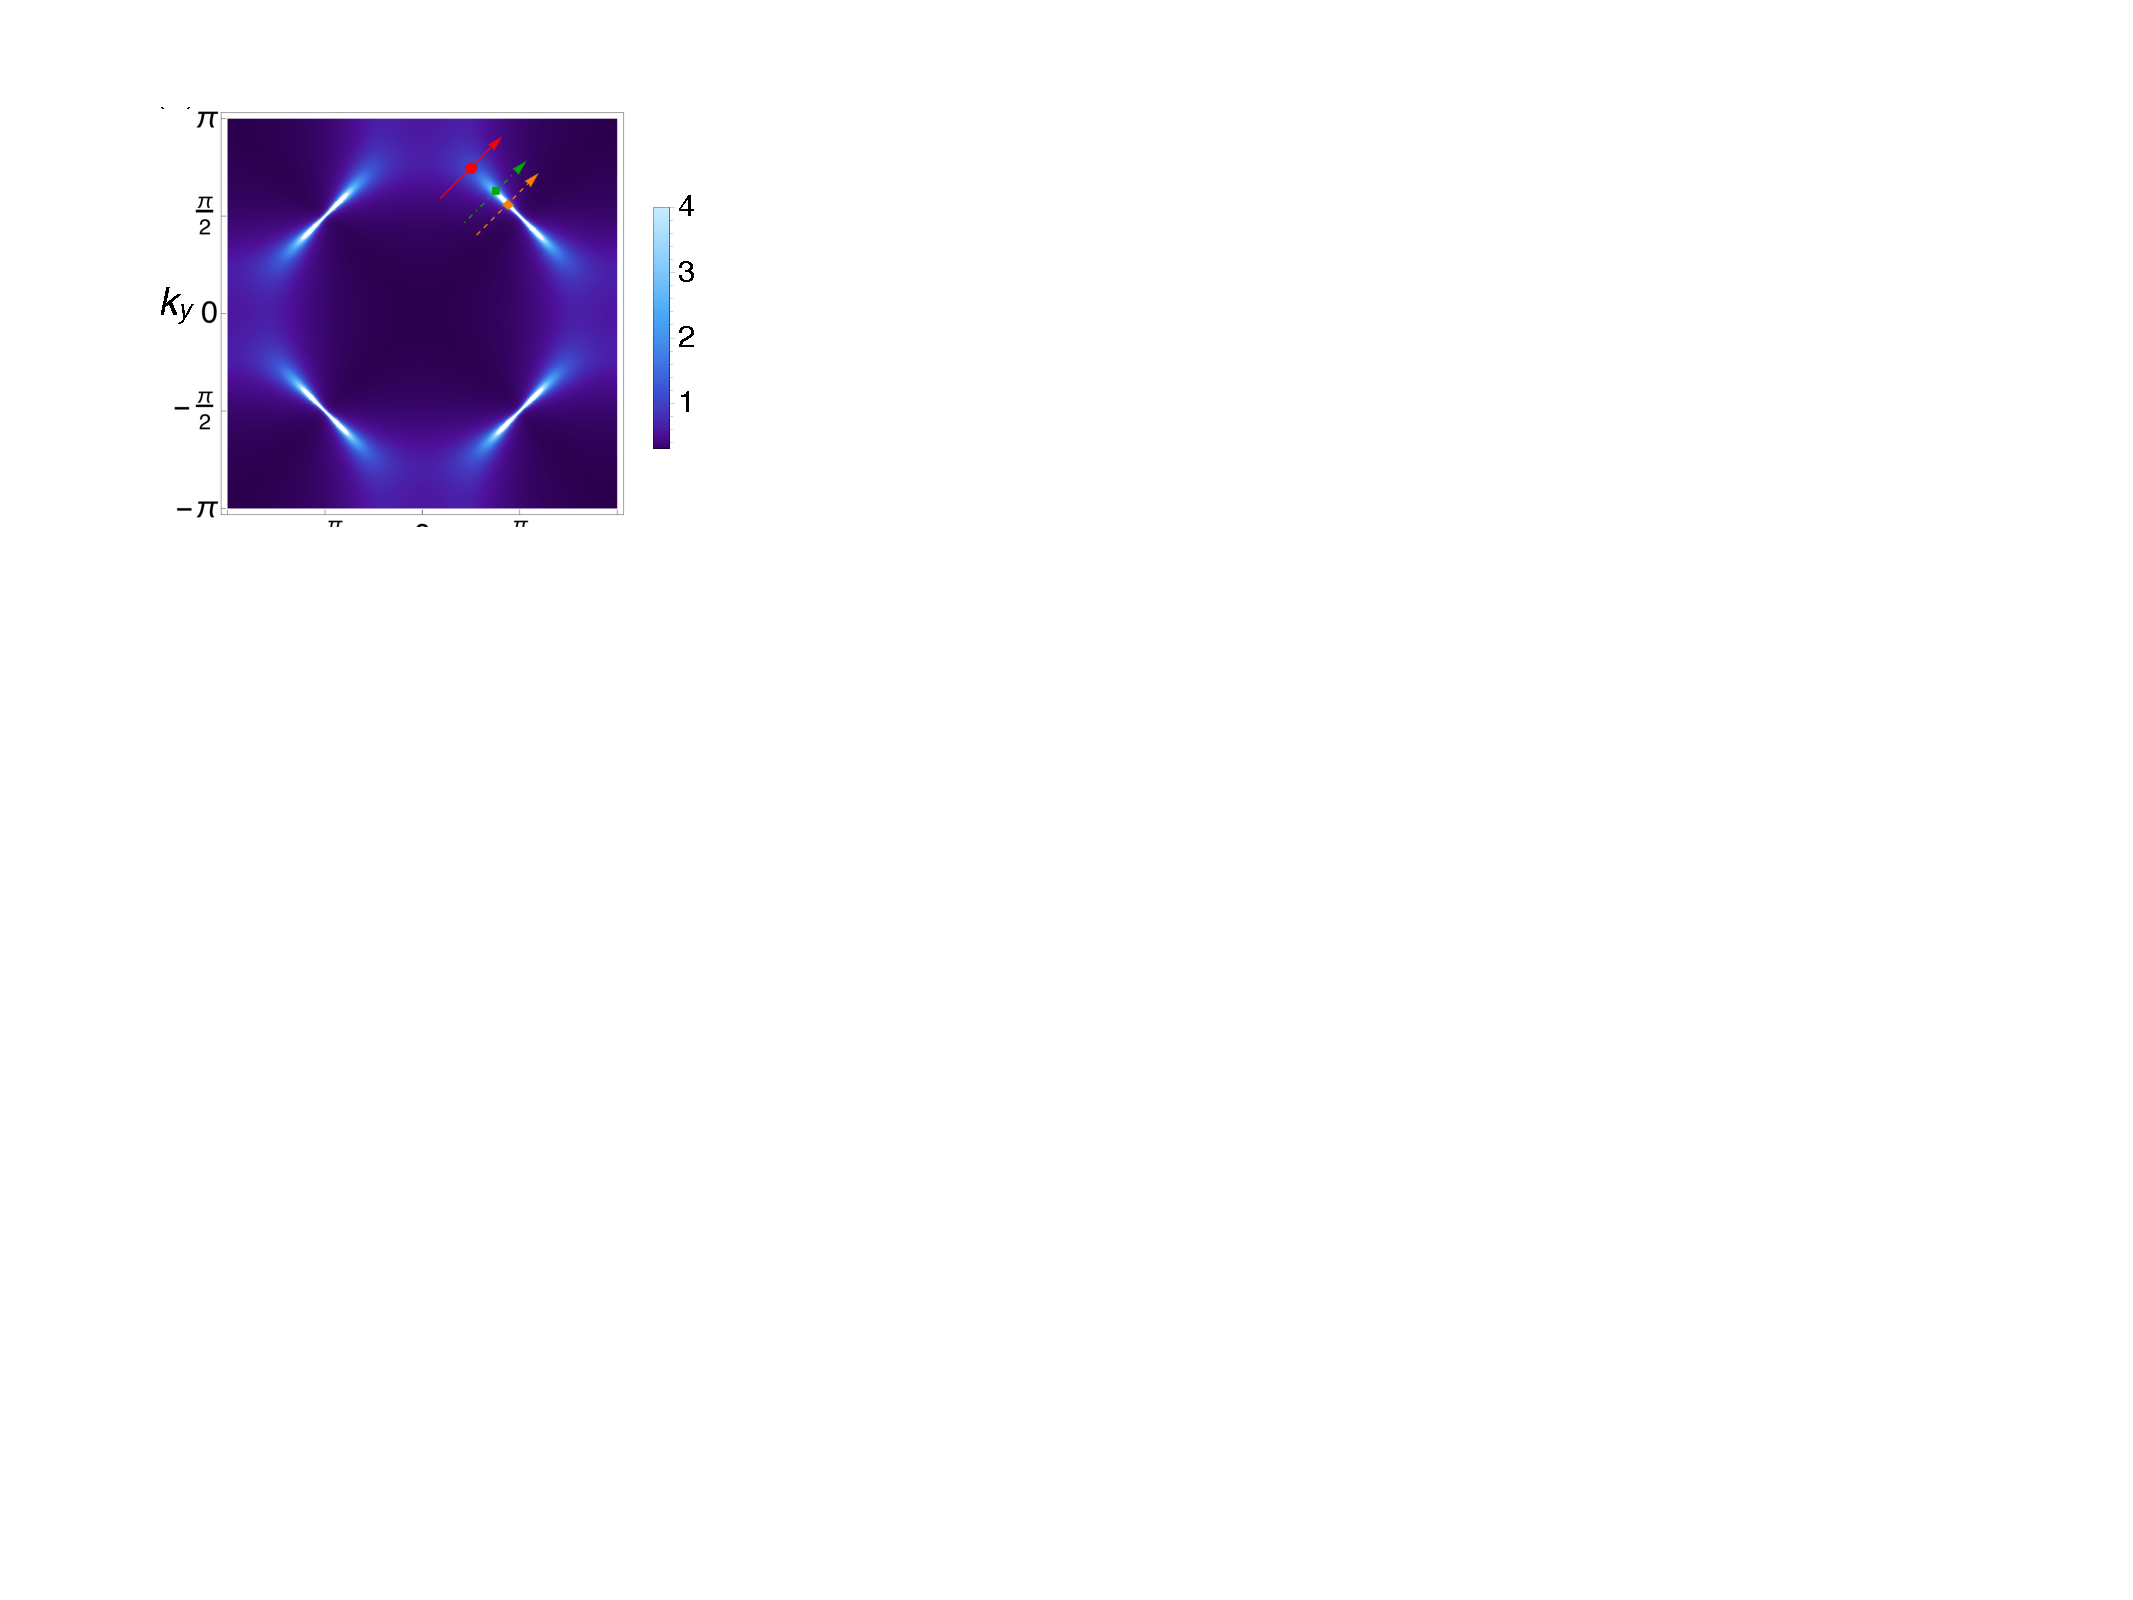
\includegraphics[height=3cm]{arc1}~~~~
	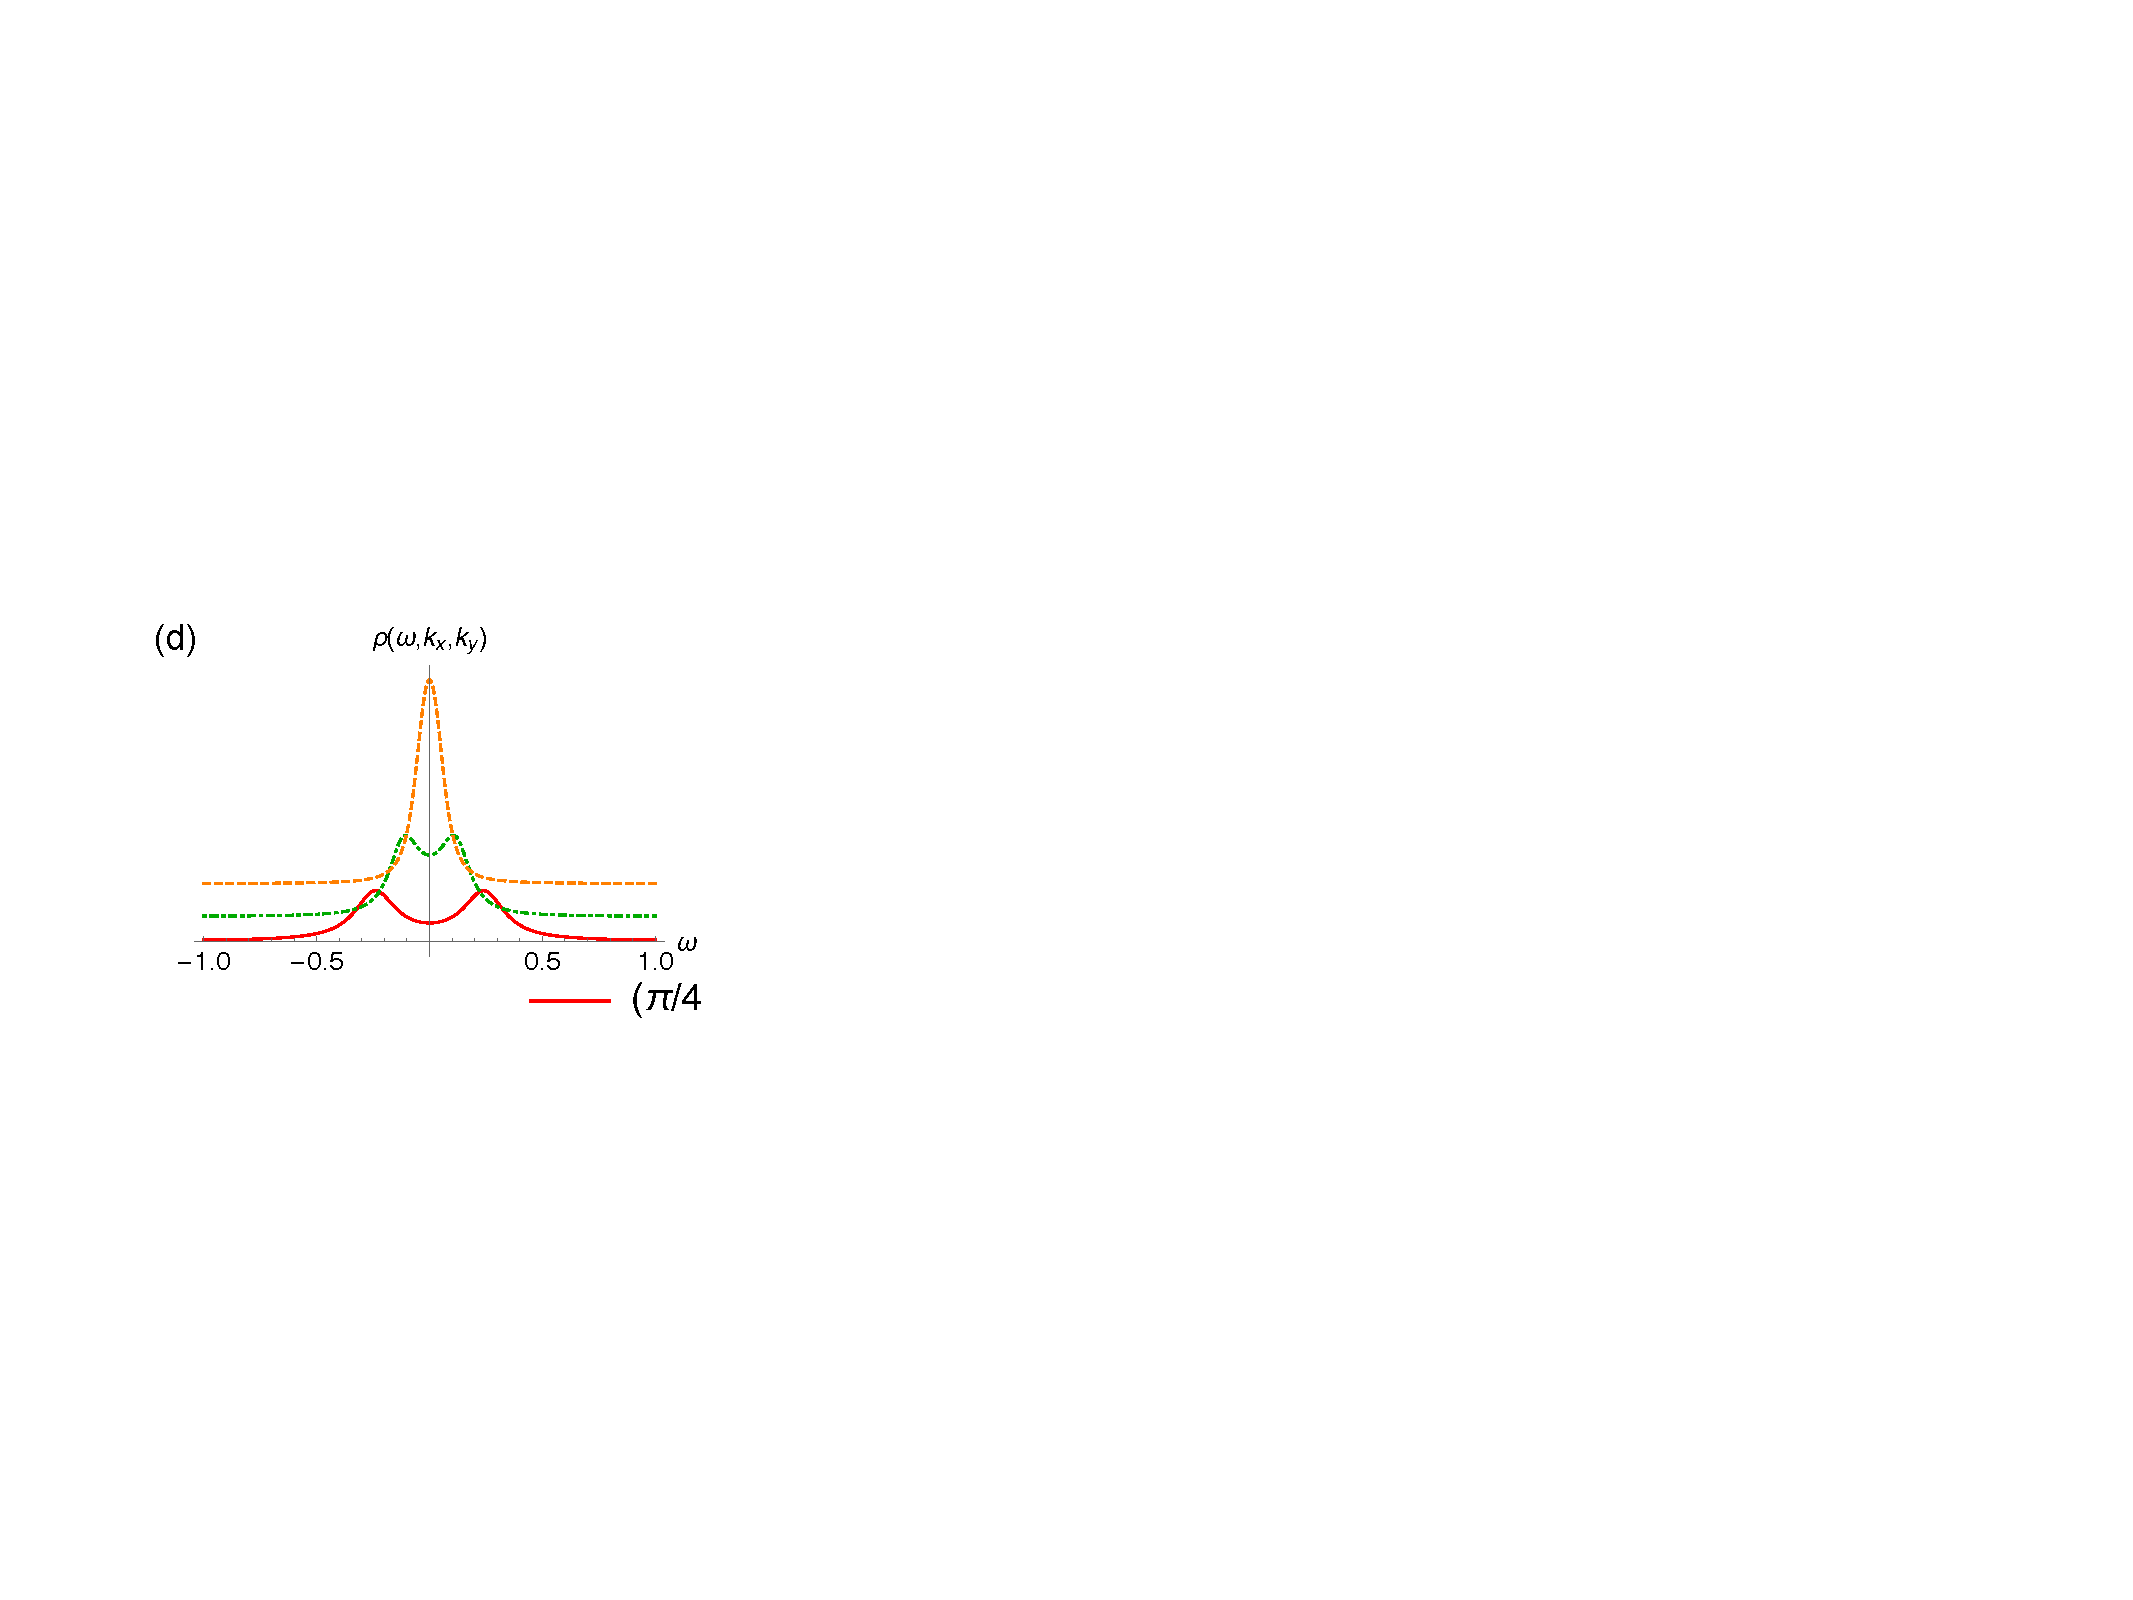
\includegraphics[height=3cm]{arc2}
\end{center}
\end{frame}

%\section{Fermi Arcs}

%\section{Conclusion}

\end{document}
